\chapter{Contextualização}
\label{chap:contextualizacao}

Este capítulo dá uma visão geral sobre os trabalhos relacionados acerca de exploração de feedback, métodos de destacamento de informações e aplicação de análises temporais. Também é apresentado o sistema que está sendo estendido neste trabalho.

\section{Trabalhos Relacionados}

A literatura na análise de dados espaciais possui um foco na eficiência das iterações exploratórias. A abordagem comum é projetar índices pré-processados, os quais permitem a consulta eficiente de dados espaciais \cite{lins2013nanocubes}. No entanto, também é preciso direcionar a atenção para o {\em valor} dos dados espaciais, porque é muito comum encontrar um analista se perdendo numa enorme quantidade de pontos geográficos. Para solucionar esse problema, ambientes de visualização, como, por exemplo, Tableau\footnote{\it http://www.tableau.com}, Exhibit\footnote{\it http://www.simile-widgets.org/exhibit/}, Spotfire\footnote{\it  http://spotfire.tibco.com}, oferecem funcionalidades para manipular os dados como filtros, consultas agregadores, entre outras. Entretanto essas funcionalidades não se mostram eficazes, visto que nessas ferramentas o pesquisador precisa saber exatamente o que procura. Este trabalho combina a exploração de feedback, métodos de destacamento de informações e análise temporal a fim de otimizar a análise exploratória.

\subsection{Exploração de Feedback}

O modelo espaço-temporal proposto aprimora o processo de análise de dados espaciais destacando subconjuntos de pontos geográficos com base no feedback coletado durante a exploração do analista. Na literatura, há vários trabalhos sobre exploração de feedback para orientar o analista nas futuras iterações da análise como, por exemplo, \citeonline{boley2013one}. A abordagem comum é uma metodologia {\em top-$k$} para reduzir o escopo da consulta baseado no feedback explícito e recomendar um pequeno subconjunto de resultados interessantes de tamanho $k$. Uma clara distinção do presente trabalho é que não busca-se reduzir o escopo, mas alavancar o conjunto de dados com resultados potencialmente interessantes que o analista talvez não tenha notado devido ao enorme volume de dados espaciais. Enquanto as escolhas do analista são limitadas por $k$ em algoritmos de {\em top-$k$} processamento, a abordagem proposta oferece a liberdade de escolha ao mesmo tempo que pontos geográficos vão sendo transparentemente destacados com base nas novas escolhas do analista.

\subsection{Métodos de Destacamento de Informação}

\todo{fala de cada um}

Há trabalhos na literatura sobre métodos de destacamento de informações, por exemplo: \citeonline{Liang2010,Robinson2011,wongsuphasawat2016voyager,willett2007scented}. Entretanto todos esses métodos são {\em objetivos} e não são aplicáveis para o contexto de orientação espacial onde o feedback do usuário é envolvido. Em termos de recomendação, algumas abordagens focam na dimensão espacial \cite{Bao2015,Levandoski:2012} enquanto o contexto e a diversidade do resultado é deixado de lado.

\subsection{Aplicações de Análise Temporal}

Existem várias instâncias na literatura que combinam análise temporal com dados espaciais, como \citeonline{baculo2017,balahadia2017,chidean2018,ghahramani2018,kamath2013,lopestexeira2018,ma2017,mijovic2016,tomoki2010,nara2007,zhan2017,zheng2018}. Essas aplicações de análise temporal são em contextos específicos, os quais não envolvem feedback do usuário, mas representam como análise temporal pode ser perspicaz e proveitosa.

\citeonline{baculo2017} e \citeonline{balahadia2017} fazem uso de dados públicos de Manila, capital das Filipinas, combinando dados espaciais, análise temporal e modelos preditivos e mostrando resultados que podem ser utilizados para preparação de um plano de gestão pública eficaz. \citeonline{ma2017} e \citeonline{zheng2018} também fazem análises realistas de como eventos, como protestos, impactam nas trajetórias de táxis, cujos resultados podem auxiliar no controle de tráfego urbano e nos planos de serviços de transporte da cidade. Ambos realizam ricas análises, as quais contribuíram como inspiração neste trabalho.

\citeonline{chidean2018} apresenta como detectar padrões espaço-temporais no contexto do uso de energia eólica na Península Ibérica usando o algoritmo {\em Second-Order Data-Coupled Clustering}. Apesar do estudo detalhado, esse trabalho não contempla um contexto de análise exploratória.

\citeonline{ghahramani2018}, \citeonline{lopestexeira2018} e \citeonline{zhan2017} demonstram como análise temporal pode ser aplicada no contexto geográfico. \citeonline{zhan2017} vai além gerando uma árvore de clusterização hierárquica. Apesar dos métodos e resultados serem bem detalhados nos trabalhos, essas contribuições não se aplicam ao assunto em questão.

\citeonline{kamath2013} propõe uma abordagem de {\em reinforcement learning} para prever eventos (adoção de {\em memes}) num contexto espaço-temporal. \citeonline{nara2007} introduz um modelo de visualização 3D para dados espaço-temporais que ajuda a analisar qualitativa e quantitativamente os padrões e tendências espaço-temporais. Ambos os trabalhos contribuem para representar como o modelo proposto pode ser combinado com diversas técnicas.

\section{GeoGuide}

\begin{figure}[t]
	\centering
	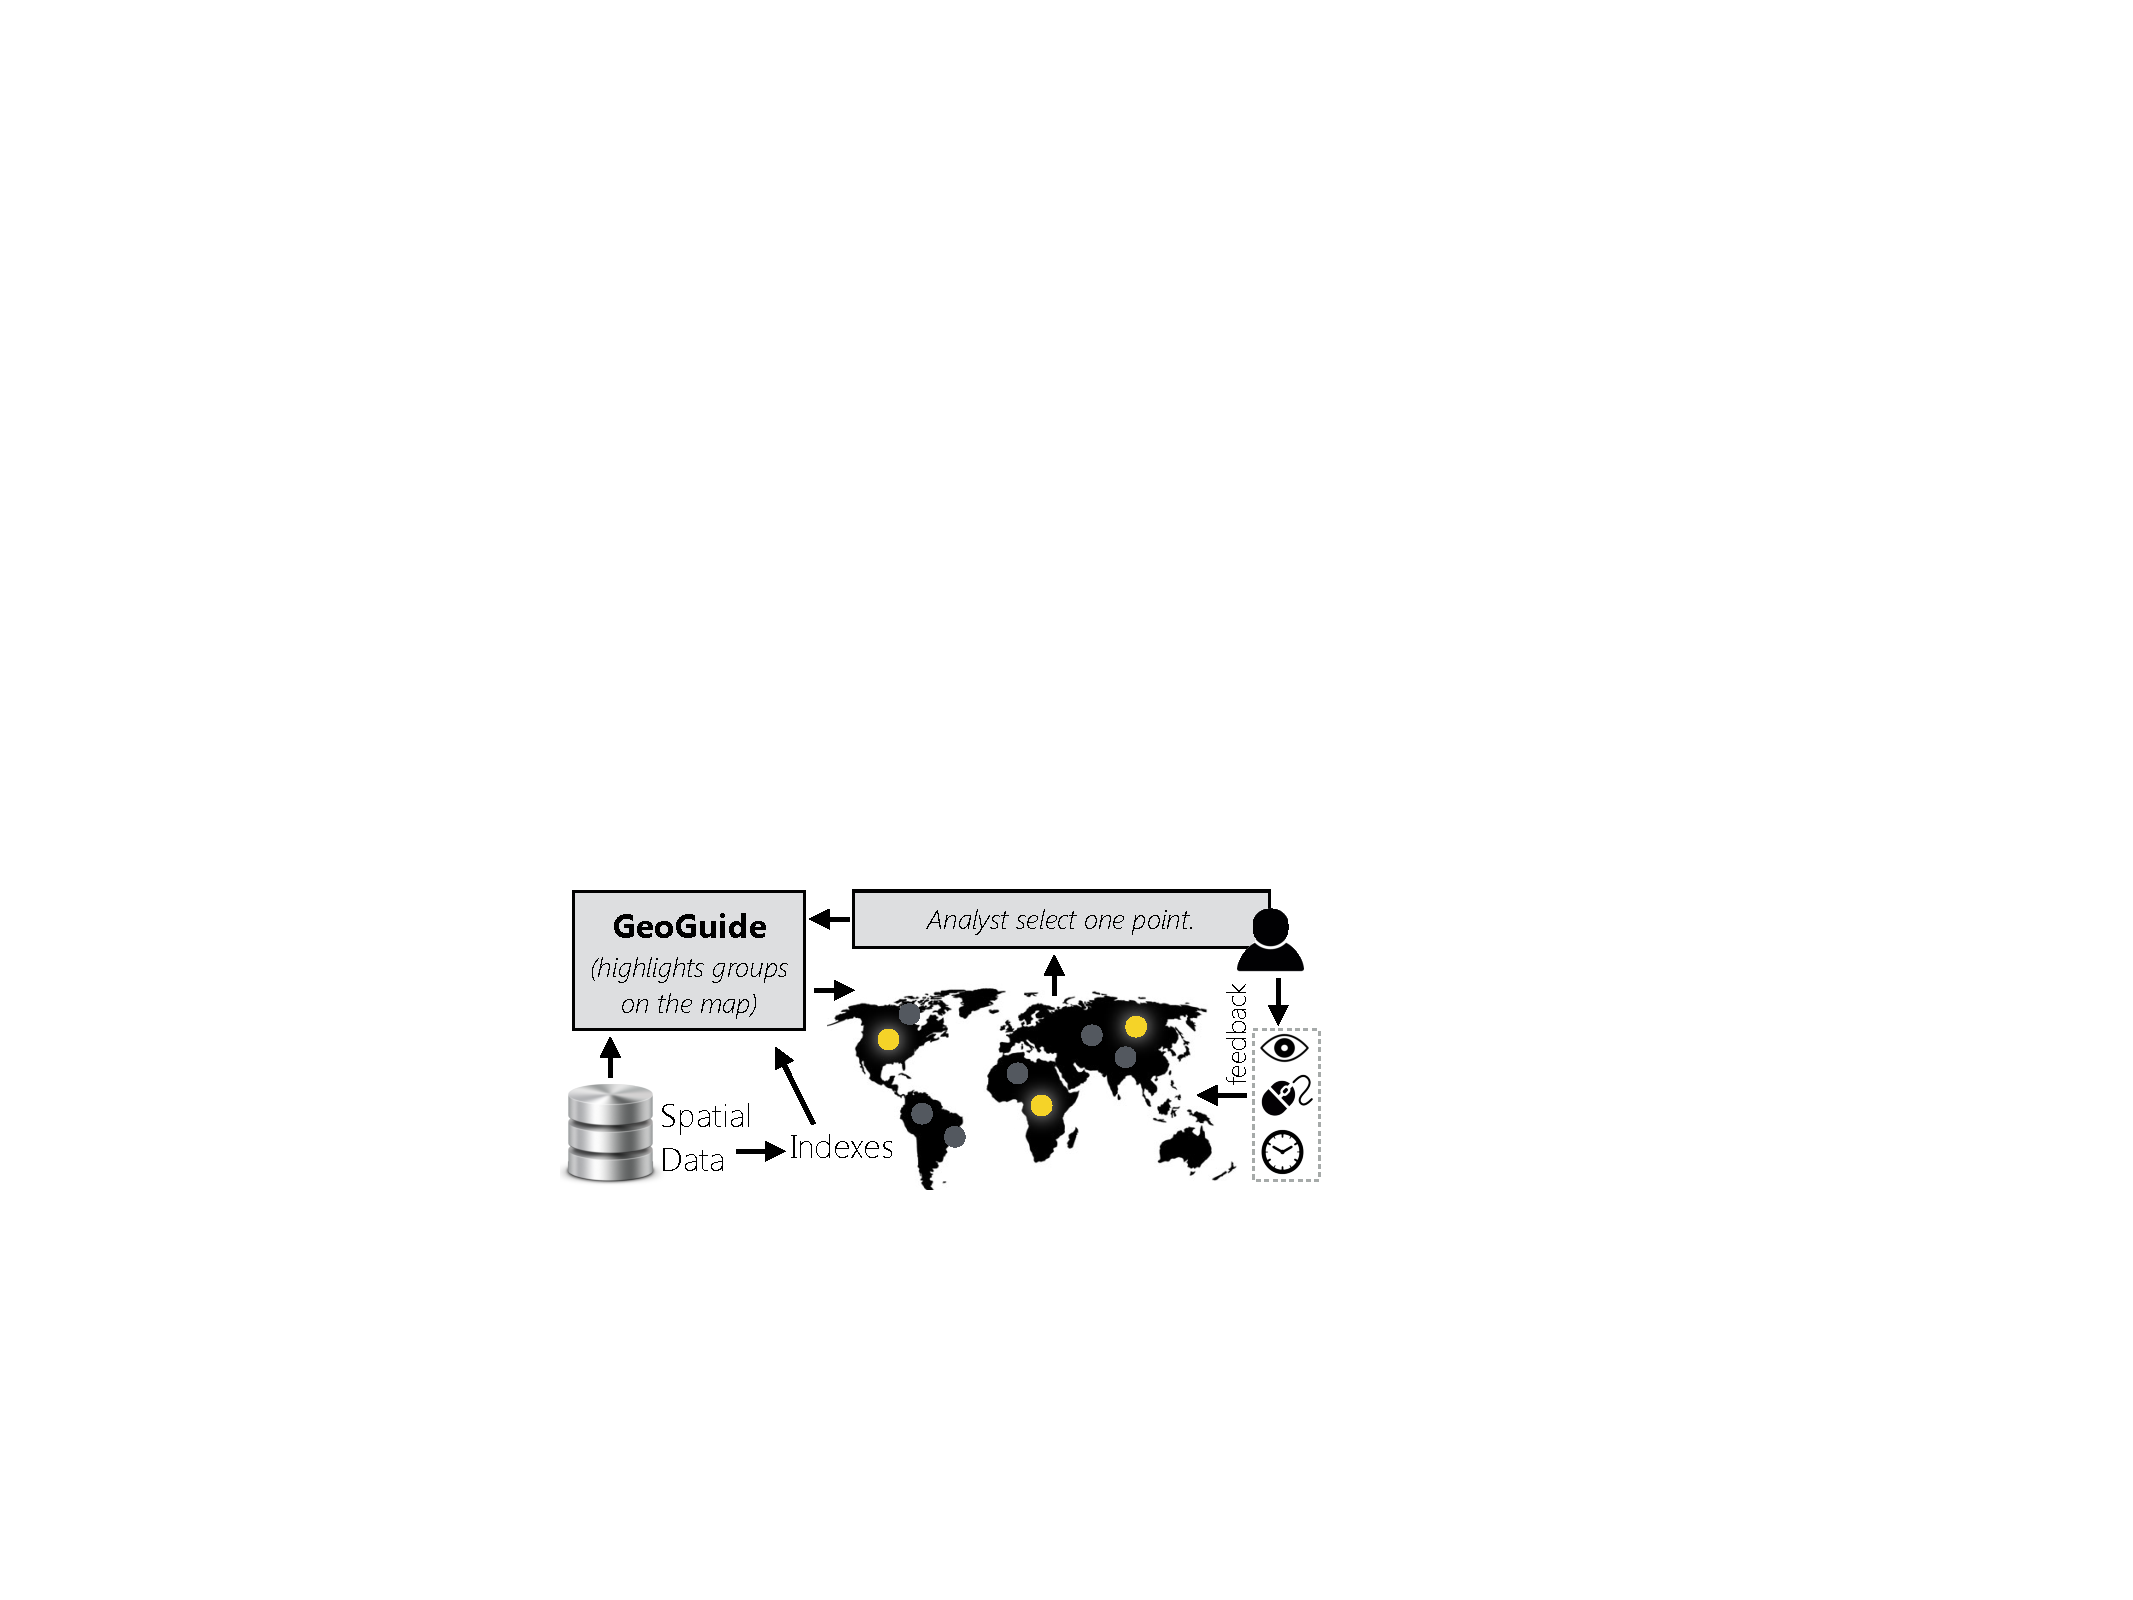
\includegraphics[width=\columnwidth]{imagens/framework}
	\caption{Componentes do GeoGuide}
	\label{fig:framework}
	\vspace{-10pt}
\end{figure}

\abrv[TADS -- Tecnologia em Análise e Desenvolvimento de Sistemas]{}
\abrv[IFRN -- Instituto Federal do Rio Grande do Norte]{}

GeoGuide \cite{omidvarTehrani2017} é fruto de um projeto de pesquisa realizado por alunos do curso de Tecnologia em Análise e Desenvolvimento de Sistemas (TADS) no Instituto Federal do Rio Grande do Norte (IFRN) em colaboração com a Universidade de Grenoble. Esse projeto se trata de um ambiente de visualização de dados espaciais que coleta as preferências do usuário durante a exploração para destacar subconjuntos de pontos geográficos que podem ser interessantes ao analista. Figura \ref{fig:framework} ilustra os principais componentes da arquitetura do GeoGuide explorados nas próximas subseções.

Neste trabalho, o GeoGuide é potencializado à dois novos conceitos: $i$. regiões densas interessantes e $ii$. análise temporal das preferências do usuário. Esses dois conceitos serão explorados no próximo capítulo.

\subsection{Pré-processamento}

GeoGuide realiza um passo de pré-processamento para criar os índices que serão usados durante a fase de destacamento. O índice é uma tabela comparativa entre todos os pontos usando duas métricas de qualidade: relevância e diversidade. Os valores calculados são normalizados no intervalo de $0.0$ à $1.0$.

\subsubsection{Relevância e Diversidade}

\begin{figure}[t]
	\centering
	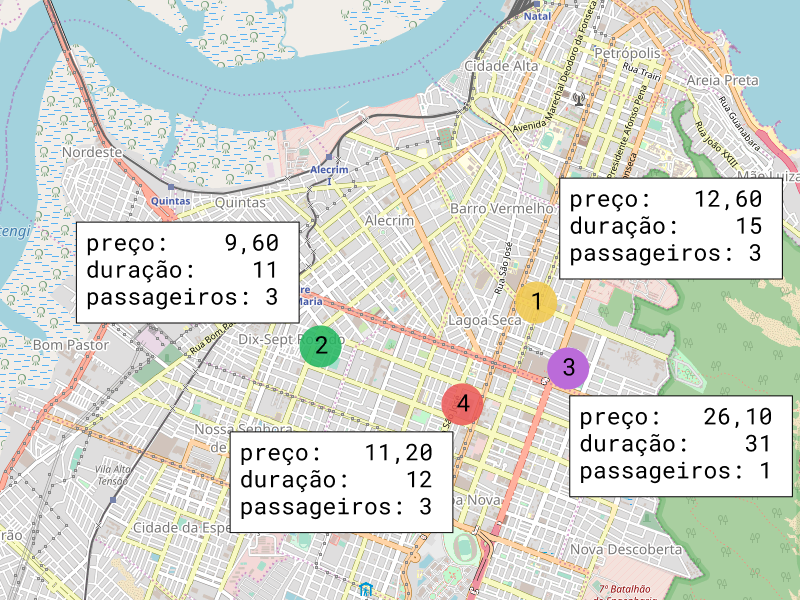
\includegraphics[width=\columnwidth]{imagens/exemplo-de-pontos}
	\caption{Exemplo de pontos geográficos com seus atributos}
	\label{fig:exemplo-pontos}
	\vspace{-10pt}
\end{figure}

Relevância representa o quão similar é o ponto $a$ com o ponto $b$ num conjunto de dados. GeoGuide usa a relevância para destacar pontos similares ao feedback do analista. Diversidade representa quão distante o ponto $a$ está localizado do ponto $b$. GeoGuide usa a diversidade para permitir ao analista explorar diferentes regiões, mas ainda assim trabalhar com pontos relevantes ao seu interesse.

\begin{table}[!h]
	\centering
	\begin{tabular}{|c|c|r|r|}
	\hline
	\multicolumn{1}{|c|}{\textbf{Ponto A}} & \multicolumn{1}{c|}{\textbf{Ponto B}} & \multicolumn{1}{c|}{\textbf{Relevância}} & \multicolumn{1}{c|}{\textbf{Diversidade}} \\ \hline
	1                                      & 2                                     & 0.8                                      & 0.9                                       \\ \hline
	1                                      & 3                                     & 0.25                                     & 0.2                                       \\ \hline
	1                                      & 4                                     & 0.9                                      & 0.45                                      \\ \hline
	2                                      & 3                                     & 0.2                                      & 1.0                                       \\ \hline
	2                                      & 4                                     & 1.0                                      & 0.48                                      \\ \hline
	3                                      & 4                                     & 0.2                                      & 0.3                                       \\ \hline
	\end{tabular}
	\caption{Exemplo de Índice de Relevância e Diversidade para pontos na Figura \ref{fig:exemplo-pontos}}
	\label{table:exemplo-indice}
\end{table}

Na Figura \ref{fig:exemplo-pontos}, tem-se, por exemplo, pontos geográficos que representam viagens de táxi. Cada ponto (1, 2, 3 e 4), possui seus atributos: preço da viagem, duração da viagem e a quantidade de passageiros; e sua localização geográfica. Na tabela \ref{table:exemplo-indice}, ilustra-se o exemplo do índice calculado diante dos pontos apresentados na Figura \ref{fig:exemplo-pontos}. Percebe-se que os pontos mais similares entre si são os pontos 2 e 4, enquanto que 2 e 3 são os mais distantes, ou seja, possuem o maior valor de diversidade.


\subsection{Preferências do Usuário}

Para coletar as preferências do usuário, GeoGuide usa ambos feedback implícito e explícito. Feedback explícito é quando o usuário está analisando os atributos de um ponto, por exemplo a descrição de uma casa no Airbnb, e explicitamente pede para explorar pontos similares ao selecionado. Feedback implícito é coletado através da captura dos movimentos do mouse e métricas como  ``quanto tempo o usuário passou analisando o perfil de um ponto''.

\subsection{Destacamento de Dados Espaciais}

GeoGuide combina o índice pré-processado e o feedback coletado para destacar subconjuntos de dados espaciais de acordo com as preferências do analista. O processo de destacamento provou ser eficiente em termos de ``quantos passos o analista leva até completar a tarefa de encontrar um ponto com um determinado perfil''. Usando GeoGuide, analistas foram capazes de completar a tarefa usando, em média, 10.7 passos, enquanto que usando Tableau, foram necessários 43 passos \cite{omidvarTehrani2017}.

% \vspace{25pt}
% \endsubsection

% \closesubsection
